\documentclass[a4paper]{article}
\usepackage[left=1cm, right=1cm, top=1cm, bottom=1cm]{geometry}
% put the command
%
% \input{odl_preamble.tex}
%
% at the top of your latex file (just after the \documentclass) to include this
% in your document.  Feel free to add to this file, but please consider adding
% commands and packages that are specific to your work outside of this file:
% let's reserve this file for stuff that most of us would need.

% The amssymb package provides various useful mathematical symbols
\usepackage{amsmath}
\usepackage{amsfonts}
\usepackage{amssymb}
\usepackage{amsthm}
\usepackage{graphicx} % for includegraphics
\usepackage{xspace} % needed for \eg, \ie, \etc
\usepackage{bm} % for bold math
%\usepackage{threeparttable} % for tables with footnotes
\usepackage{subcaption}
\usepackage{caption}
\usepackage{graphicx}
\usepackage{fullpage}
\usepackage{textcomp}
\usepackage{listings}
\usepackage{xcolor}
\usepackage{float}
\usepackage{stmaryrd}
\usepackage[toc,page]{appendix}

\usepackage[ruled,lined,linesnumbered]{algorithm2e}

% hyperref must be last
\usepackage{hyperref}
\hypersetup{
  colorlinks=true,
  linkcolor=red,
  citecolor=green,
  urlcolor=blue
}
  
% We often use mathcal for functions
\newcommand{\fnc}[1]{\ensuremath{\mathcal{#1}}}
\newcommand{\vecfnc}[1]{\ensuremath{\boldsymbol{\mathcal{#1}}}} % vector function

% matrices are often math sans serif type
\newcommand{\mat}[1]{\ensuremath{\mathsf{#1}}}

\newcommand{\Pm}[0]{\psi_h^{(n-1)}}
\newcommand{\Pn}[0]{\psi_h^{(n)}}
\newcommand{\Pnn}[0]{\psi_h^{(n+1)}}
\newcommand{\Qn}[0]{q_h^{(n)}}
\newcommand{\Qnn}[0]{q_h^{(n+1)}}

\newcommand{\Sn}[0]{s_h^{(n)}}
\newcommand{\Snn}[0]{s_h^{(n+1)}}
\newcommand{\Lht}[0]{L_{h,\Delta t}}

% SBP operator matrices
\newcommand{\M}[0]{\mat{M}}
\newcommand{\Dx}[0]{\mat{D}_{x}}
\newcommand{\Dy}[0]{\mat{D}_{y}}
\newcommand{\Dz}[0]{\mat{D}_{z}}
\newcommand{\Sx}[0]{\mat{S}_{x}}
\newcommand{\Sy}[0]{\mat{S}_{y}}
\newcommand{\Sz}[0]{\mat{S}_{z}}
\newcommand{\Qx}[0]{\mat{Q}_{x}}
\newcommand{\Qy}[0]{\mat{Q}_{y}}
\newcommand{\Qz}[0]{\mat{Q}_{z}}
\newcommand{\Ex}[0]{\mat{E}_{x}}
\newcommand{\Ey}[0]{\mat{E}_{y}}
\newcommand{\Ez}[0]{\mat{E}_{z}}
\newcommand{\Par}[2]{\frac{\partial {#1}}{\partial{#2}}}
% optimization commands
\newcommand{\Lag}[0]{\fnc{L}}
\newcommand{\optmin}{\ensuremath{\text{minimize}}}
\newcommand{\wrt}{\ensuremath{\text{with respect to}}}
\newcommand{\st}[0]{\ensuremath{\text{s.t.}}}
\newcommand{\W}[0]{\mat{W}} % Hessian
\newcommand{\A}[0]{\mat{A}} % Jacobian
\newcommand{\K}[0]{\mat{K}} % KKT matrix
\newcommand{\Hess}[0]{\mat{H}} % upper Hessenberg
\newcommand{\I}[0]{\mat{I}} % identity
\newcommand{\diff}[0]{\mathrm{d}}
% common math operators
\DeclareMathOperator{\spn}{span}
\DeclareMathOperator{\range}{range}
\DeclareMathOperator{\mydiag}{diag}
\newcommand{\argmin}[0]{\ensuremath{\operatornamewithlimits{argmin}}}
\newcommand{\sgn}[0]{\operatorname{sgn}}
\newcommand{\nullsp}[0]{\operatorname{null}}

% environments for definitions, therorems, etc 
\newtheorem{definition}{Definition}
\newtheorem{proposition}{Proposition}
\newtheorem{corollary}{Corollary}
\newtheorem{lemma}{Lemma}
\newtheorem{remark}{Remark}
\newtheorem{assumption}{Assumption}
\newtheorem{thrm}{Theorem}

% command latin phrases and other short-forms
\newcommand{\etal}[0]{{\em et~al.\@}\xspace}
\newcommand{\eg}[0]{{e.g.\@}\xspace}
\newcommand{\ie}[0]{{i.e.\@}\xspace}
\newcommand{\viz}[0]{{viz.\@}\xspace}
\newcommand{\resp}[0]{{resp.\@}\xspace}

\newcommand{\Jump}[1]{\llbracket #1\rrbracket}
\newcommand{\Mean}[1]{\{\{#1\}\}}
% Misc. commands
\newcommand{\ignore}[1]{} % comment out large sections of code


\title{Assignment 4: Adjoint of unsteady 1D Euler Equations}
\author{Jianfeng Yan}
\begin{document}
 \maketitle
 
\begin{abstract}
  
\end{abstract}

\section{Summary}
For this assignment, the following functionalities have been implemented:
\begin{itemize}
  \item derived the continuous adjoint equation of unsteady 1D Euler equation given the specific functional;
  \item derived the discrete adjoint equation of unsteady 1D Euler with Crank-Nicolson discretization;
  \item solved the unsteady adjoint equation;
  \item computed the total derivative of the functional with respect to the source using adjoint variable.
\end{itemize}
\subsection{How to run the code}
\hspace{1cm}\texttt{julia assign4\_example.jl}\\
Note to turn on the finite difference verification of $DJ/Ds$, just change value of \texttt{FD\_verification} to \texttt{true}.
\section{Continuous adjoint equation}

We first derive the Frechet derivative for the nonlinear differential operator $N(q) = \Par{F}{x}$:
\begin{equation}
\begin{aligned}
N'[q]w &= [\frac{\partial}{\partial \epsilon}
\Par{F(q+\epsilon w)}{x}]_{\epsilon=0} 
= \Par{(Aw)}{x}
\end{aligned}
\end{equation}
where $A=\Par{F}{q}$ is the flux Jacobian matrix. This is
followed by the corresponding adjoint differential operator:
\begin{equation}
\begin{aligned}
(\psi, N'[q]w)_{\Omega} &= \int_{\Omega} \psi^T (\Par{Aw}{x})\diff\Omega  \\
&= -\int_{\Omega} w^TA^T\Par{\psi}{x}\diff\Omega + \int_{\partial\Omega}w^TA^T\psi\diff\Gamma \\
&= -\int_{\Omega} w^TA^T\Par{\psi}{x}\diff\Omega +  \int_{\partial\Omega}w^TA^T\psi\diff\Gamma \\
&= -\int_{0}^{1} w^TA^T\Par{\psi}{x}\diff x + [w^T A^T\psi]|_{x=1} - [w^T A^T\psi]|_{x=0}
\end{aligned}
\end{equation}
Then we derive the Frechet derivative of the functional:
\begin{equation}
J'[q]w = \int_{0}^{2}\int_{0}^{1}w^T \kappa(p-p_{targ})p'[q] \diff x\diff t
\end{equation}



By definition, the Lagrangian is 
\begin{equation}
\begin{aligned}
L &= J(q) - \int_{0}^{2}(\psi, R(q))_{\Omega}dt - \int_{0}^{2}[\psi^TA (q-q(0,t))]|_{x=0}\diff t - \int_{0}^{1}[\psi^T(q - q(x,0))]_{t=0}\diff x\\
\end{aligned}
\end{equation}
As can be seen, in addition to the primal PDE, we have also involved the boundary conditions and the initial conditions.
Taking the derivative of the Lagrangian with a variant $w$, we get
\begin{equation}
\begin{aligned}
L'[q]w &= J'[q]w - \int_{0}^{2}(\psi, R'[q]w)_{\Omega} dt - \int_{0}^{2}[w^TA^T\psi]_{x=0}\diff t - \int_{0}^{1}[w^T\psi]_{t=0}\diff x\\
&= J'[q]w - \int_{0}^{2}(\psi, \Par{w}{t} + N'[q])w)_{\Omega} dt - \int_{0}^{2}[w^TA^T\psi]_{x=0}\diff t - \int_{0}^{1}[w^T\psi]_{t=0}\diff x\\
&=  \int_{0}^{2}\int_{0}^{1}w^T \kappa(p-p_{targ})p'[q]\diff x\diff t + \int_{0}^{2}\int_{0}^{1}w^T \Par{\psi}{t}\diff x\diff t - \int_{0}^{1}[w^T\psi]|_{t=2}\diff x \\
&+ \int_{0}^{2} \int_{0}^{1}w^T A^T\Par{\psi}{x}\diff x\diff t - \int_{0}^{2} [w^TA^T \psi]_{x=1}\diff t\\
&= \int_{0}^{2}\int_{0}^{1} w^T(\Par{\psi}{t} + A^T\Par{\psi}{x} + \kappa(p-p_{targ}p'[q]))\diff x \diff t \\
&-\int_{0}^{1}[w^T\psi]_{t=1}\diff x
- \int_{0}^{2} [w^TA^T \psi]_{x=1}\diff t \\
\end{aligned}
\end{equation}
By the definition of duality, all three terms should vanish since the variant $w$ is involved in these three terms. This leads to the continuous adjoint problem:\
\begin{equation}\label{eq:con_adj}
\begin{aligned}
\Par{\psi}{t}+A^T\Par{\psi}{x} + \kappa(p-p_{targ})p'[q] &= 0, \quad &&x,t\in [0,1]\times [0,2] \\
\psi(x,2) &= 0, \quad &&x\in [0,1]\\
\psi(1,t) &= 0, \quad &&t\in [0,2]
\end{aligned}
\end{equation}

\section{Discrete adjoint}
\subsection{Derivation of discrete adjoint equation}
The residual of implicit Crank-Nicholson is 
\begin{equation}
\begin{aligned}
\hat{R}_h^{(n+1)} =\M (\Qnn - \Qn) + \frac{\Delta t}{2}[R_h(\Qnn,\Snn) + R_h(\Qn, \Sn)], \quad n=0,\dots,N-1
\end{aligned}
\end{equation}
The functional is discretized as
\begin{equation}
\begin{aligned}
J_h = \sum_{n=0}^{N} w_n \Delta t\int_{0}^{1} \frac{1}{2}\kappa(p^{(n)} - p_{targ})^2\diff x = \sum_{n=0}^{N} w_n \Delta t g_n
\end{aligned}
\end{equation}
where $g_n = \int_{0}^{1}\frac{1}{2}\kappa(p^{(n)} - p_{targ})^2\diff x$, and $w_n$ is the weight coefficient:
\begin{equation}
w_n = \begin{cases}
1\qquad 0 < n< N\\
0.5 \qquad n=0\text{ or } n=N
\end{cases}
\end{equation}
The discrete Lagrangian is defined by subtracting the adjoint-weighted residual from the functional:
\begin{equation}\label{eq:lagr}
\begin{aligned}
\Lht &= \sum_{n=0}^{N}\Delta t w_n g_n - \sum_{n=0}^{N-1}(\Pnn)^T \hat{R_h}^{(n+1)} \\
&=\sum_{n=0}^{N}\Delta t w_n g_n - \sum_{n=0}^{N-1}(\Pnn)^T (\M (\Qnn - \Qn) + \frac{\Delta t}{2}[R_h(\Qnn,\Snn) + R_h(\Qn, \Sn)])
\end{aligned}
\end{equation} 

The discrete adjoint can be found by setting the derivative of the Lagrangian with respect to the primal solution $\Qn$ to zero. For $n=1,\dots,N-1$, we have
\begin{equation}\label{eq:deriv1}
\begin{aligned}
\Par{\Lht}{\Qn} &= \Delta t w_n \Par{g_n}{\Qn} - \M^T(\Pn -  \Pnn) - \frac{\Delta t}{2}(\Par{R_h}{\Qn})^T(\Pn+\Pnn) \\
%&= \Delta t w_n \Par{g_n}{\Qn} - \M^T(\Pn -  \Pnn) - \frac{\Delta t}{2}(\Par{R_h}{\Qn})^T(\Pn+\Pnn) \\
\end{aligned}
\end{equation}
For $n=N$, we have
\begin{equation}\label{eq:deriv2}
\begin{aligned}
\Par{\Lht}{q^{(N)}_h} 
&= \Delta t w_N \Par{g_N}{q^{(N)}_h} - \M^T\psi^{(N)}_h - \frac{\Delta t}{2}(\Par{R_h}{q^{(N)}_h})^T\psi^{(N)}_h \\
\end{aligned}
\end{equation}

Hence, the discrete adjoint equations are as follows
\begin{equation} \label{eq:discrete_adj}
\begin{aligned}
\M^T(\Pn -  \Pnn) + \frac{\Delta t}{2}(\Par{R_h}{\Qn})^T(\Pn+\Pnn) - \Delta t w_n \Par{g_n}{\Qn} &= 0, \quad\quad n=1\dots,N-1 \\
 \M^T\psi^{(N)}_h + \frac{\Delta t}{2}(\Par{R_h}{q^{(N)}_h})^T\psi^{(N)}_h -\Delta t w_N \Par{g_N}{q^{(N)}_h} &= 0
\end{aligned}
\end{equation}
As we can see, when $\Delta t \to 0$, the second equation in ~\eqref{eq:discrete_adj} gives $\psi^{(N)}_h \to 0$ which is consistent with the the terminal condition in ~\eqref{eq:con_adj}. For $n=1,\dots, N-1$, the temporal discretization in the adjoint equation is also Crank-Nicolson, which is second-order accurate; that is to say, the discretization is adjoint consistent.

\subsection{Results}
To solve~\eqref{eq:discrete_adj}, we do a backwards sweep: first the second equation in \eqref{eq:discrete_adj} is solved for $\psi^{(N)}$; then the first equation in \eqref{eq:discrete_adj} is solved backwards in time, \ie, $n=N-1, N-2, \dots, 0$.

\begin{figure}
  \centering
  \begin{subfigure}{0.475\textwidth}
    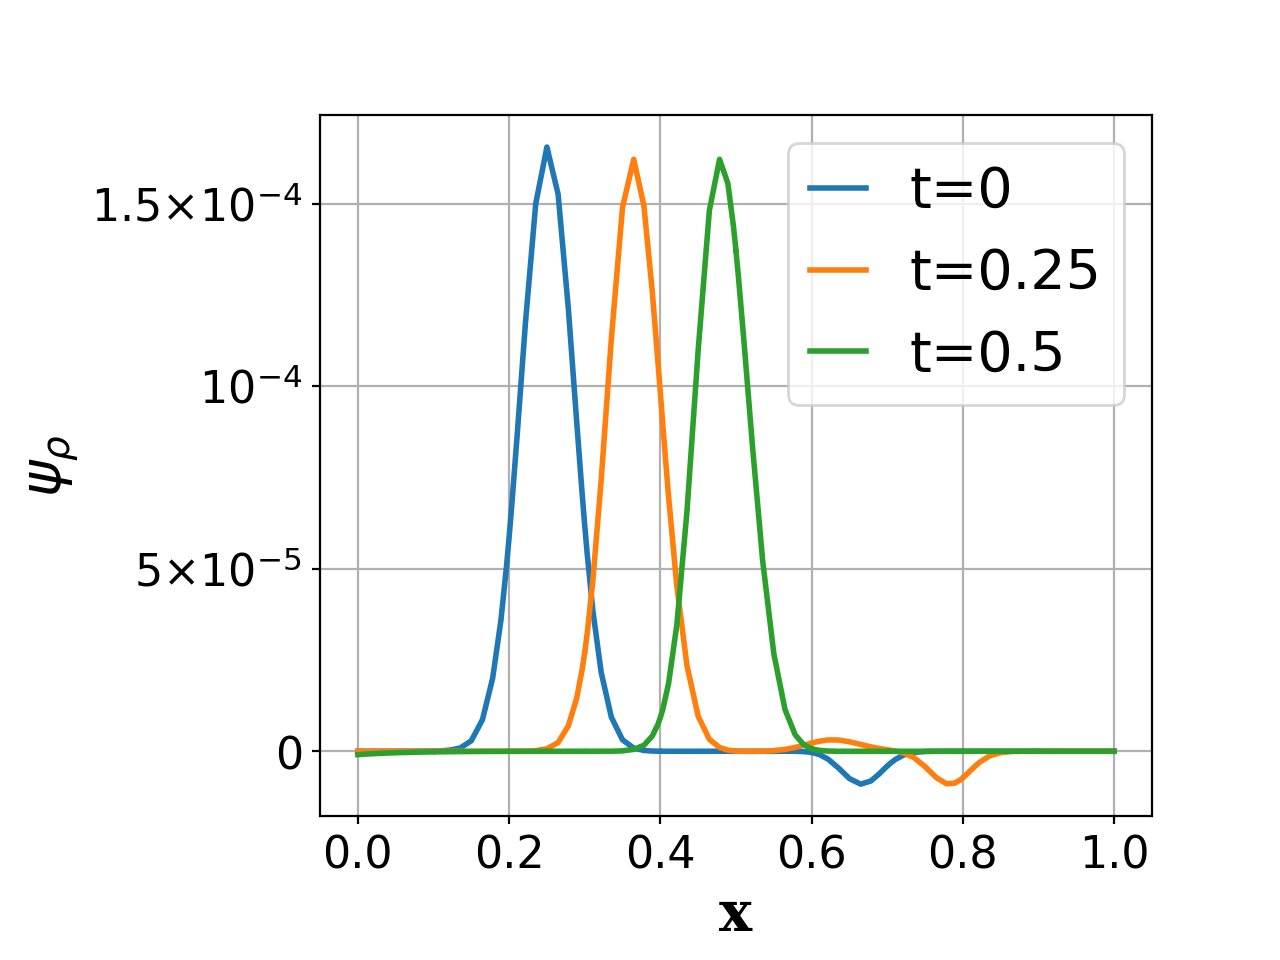
\includegraphics[width=1.0\linewidth]{figures/psi_rho.png}
    \subcaption{adjoint solution for $\rho$}
    \label{fig:psi_rho}
  \end{subfigure}
  \begin{subfigure}{0.475\textwidth}
    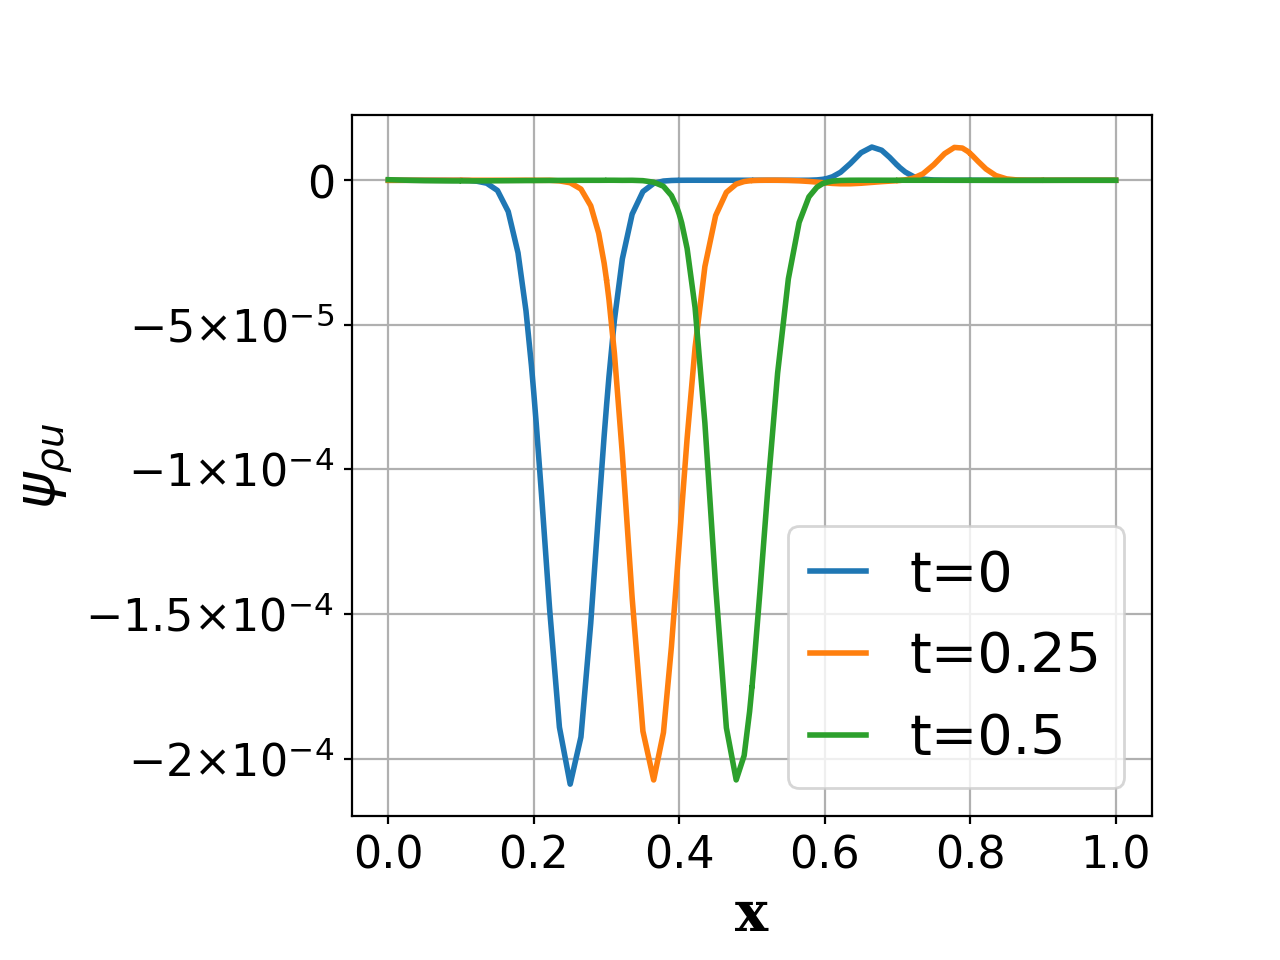
\includegraphics[width=1.0\linewidth]{figures/psi_rhou.png}
    \subcaption{adjoint solution for $\rho u$}
    \label{fig:psi_rhou}
  \end{subfigure}
  \begin{subfigure}{0.475\textwidth}
    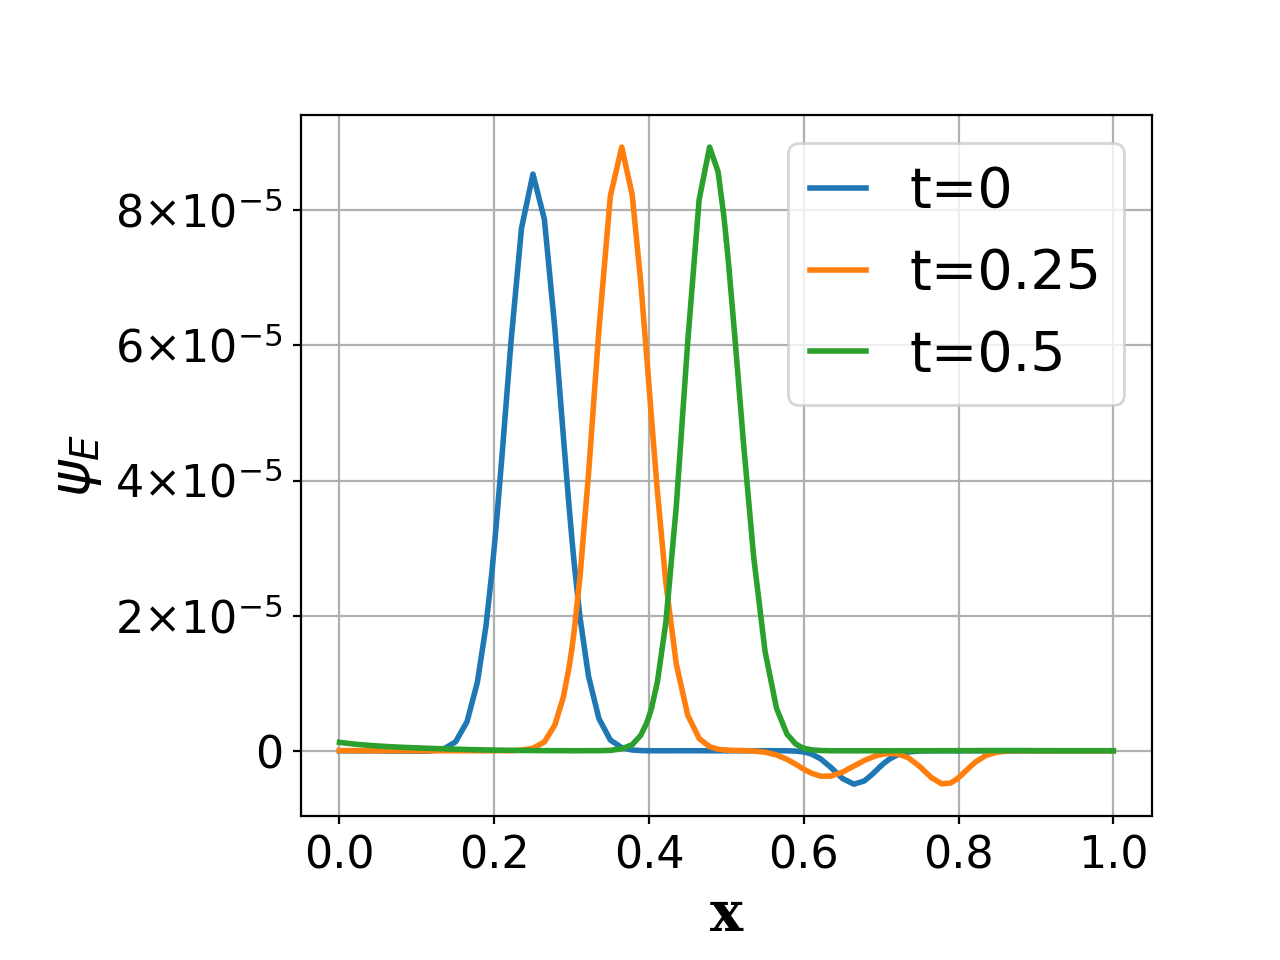
\includegraphics[width=1.0\linewidth]{figures/psi_E.png}
    \subcaption{adjoint solution for $E$}
    \label{fig:psi_E}
  \end{subfigure}
  \caption{Adjoint solution at 3 time stations}
  \label{fig:adj_distri}
\end{figure}

The following results verifies the correct derivation and implementation of the adjoint:
\begin{itemize}
  \item in Figure~\ref{fig:adj_distri} we can see the adjoint wave propagating upstream, as expected;
  \item as shown in Figure \ref{fig:adj_t=2}, the adjoint solution at $t=2$, $\psi_h(x,2)$, is nearly zero, which agrees with the terminal condition in \eqref{eq:con_adj};
  \item we will see later in Section~\ref{sec:total_deriv}, the total derivative of the functional with respect to the source obtained using adjoint-based approach matches that computed using finite difference.
  
\end{itemize}
A further verification to do would be the convergence study. 
\begin{figure}
  \centering
  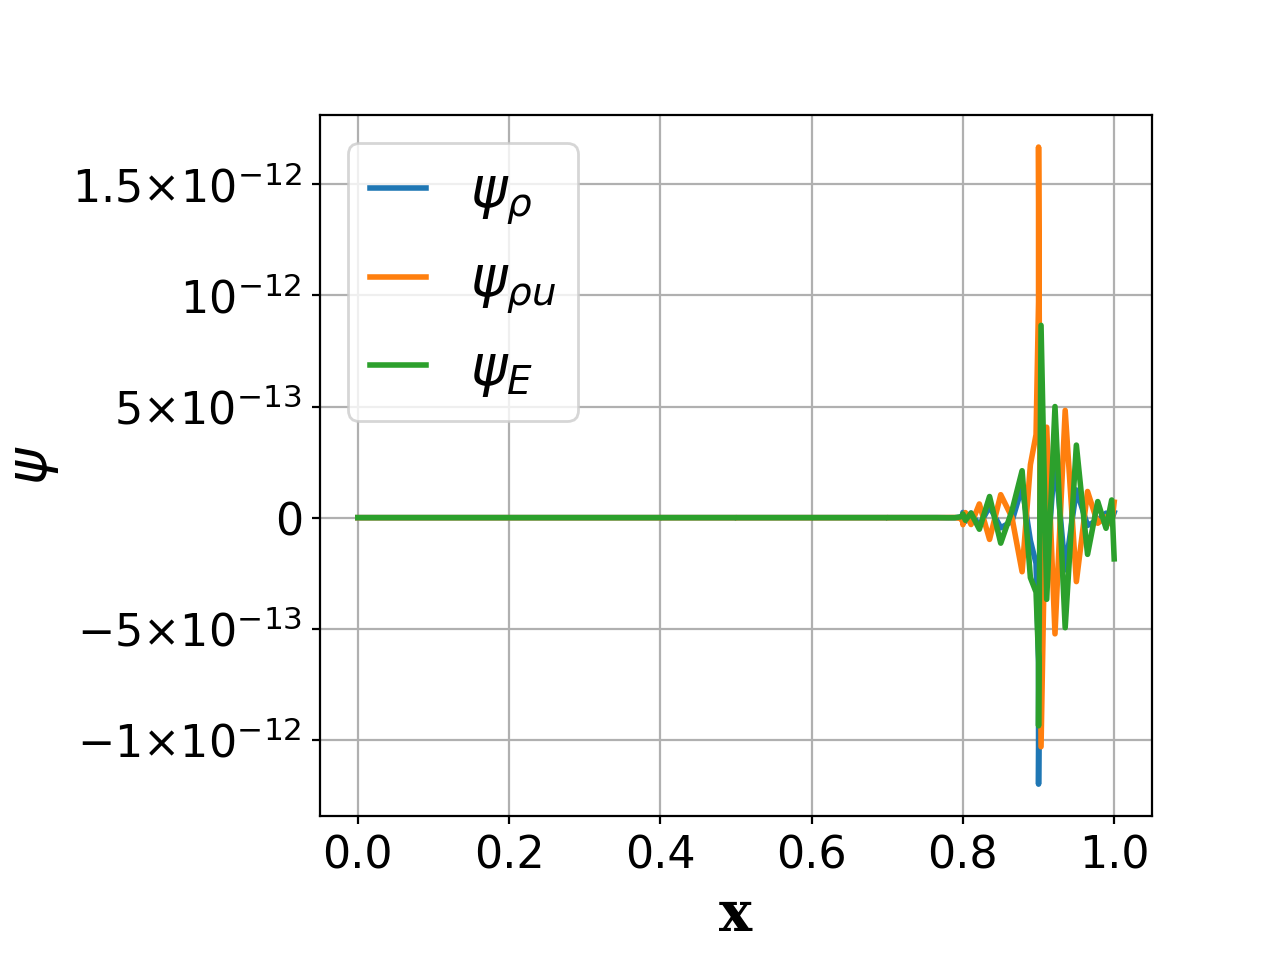
\includegraphics[width=0.5\textwidth]{figures/psi_t=2.png}
  \caption{Adjoint solution at $t=2$}
  \label{fig:adj_t=2}
\end{figure}
\section{Total derivative of functional} \label{sec:total_deriv}
According to~\eqref{eq:lagr},
\begin{equation}
\begin{aligned}
\frac{D J_h}{D s^{(i)}} &= \Par{\Lht}{s^{(i)}} \\
&= \Par{J_h}{s^{(i)}} - \sum_{n=0}^{N-1}(\Pnn)^T \Par{\hat{R}_h^{(n+1)}}{s^{(i)}} \\
&=\begin{cases}
- (\psi_h^{(i)})^T \Par{\hat{R}_h^{(i)}}{s^{(i)}} - (\psi_h^{(i+1)})^T \Par{\hat{R}_h^{(i+1)}}{s^{(i)}}, \quad 0<i<N \\
- (\psi_h^{(i+1)})^T \Par{\hat{R}_h^{(i+1)}}{s^{(i)}}, \quad i=0 \\
- (\psi_h^{(i)})^T \Par{\hat{R}_h^{(i)}}{s^{(i)}} ,\quad i=N
\end{cases}\\
&=\begin{cases}
- \frac{\Delta t}{2}(\psi_h^{(i)}+\psi_h^{(i+1)})^T \Par{R_h^{(i)}}{s^{(i)}}, \quad 0<i<N \\
- \frac{\Delta t}{2}(\psi_h^{(i+1)})^T \Par{{R}_h^{(i)}}{s^{(i)}}, \quad i=0 \\
- \frac{\Delta t}{2}(\psi_h^{(i)})^T \Par{{R}_h^{(i)}}{s^{(i)}} ,\quad i=N
\end{cases}
\end{aligned}
\end{equation}
In the above equation, we have utilized the fact that $\Par{J_h}{s^{(i)}}=0$, and that $\hat{R}_h^{(n)} = \hat{R}_h(s^{(n)}, s^{(n+1)})$ and $\Par{\hat{R}^{(n+1)}}{s^{(n)}} = \Par{\hat{R}^{(n)}}{s^{(n)}} = \frac{\Delta t}{2}\Par{R^{(n)}}{s^{(n)}}$.
We can see that in addition to the discrete adjoint variable $\Pn$, $n=1, \dots, N$, the partial derivative of the residual with respect $s$,  $\Par{\hat{R}}{s^{(n)}}$, is also required to compute the total derivative of the functional.

The result is shown in Figure~\ref{fig:dJdS}. For verification, we compare the derivatives for several time steps using adjoint-based approach to that using the finite difference method. For all time steps, the relative difference between two approaches is less than $0.02\%$, and the absolute difference is on the order of $10^{-11}$.
\begin{figure}
  \centering
  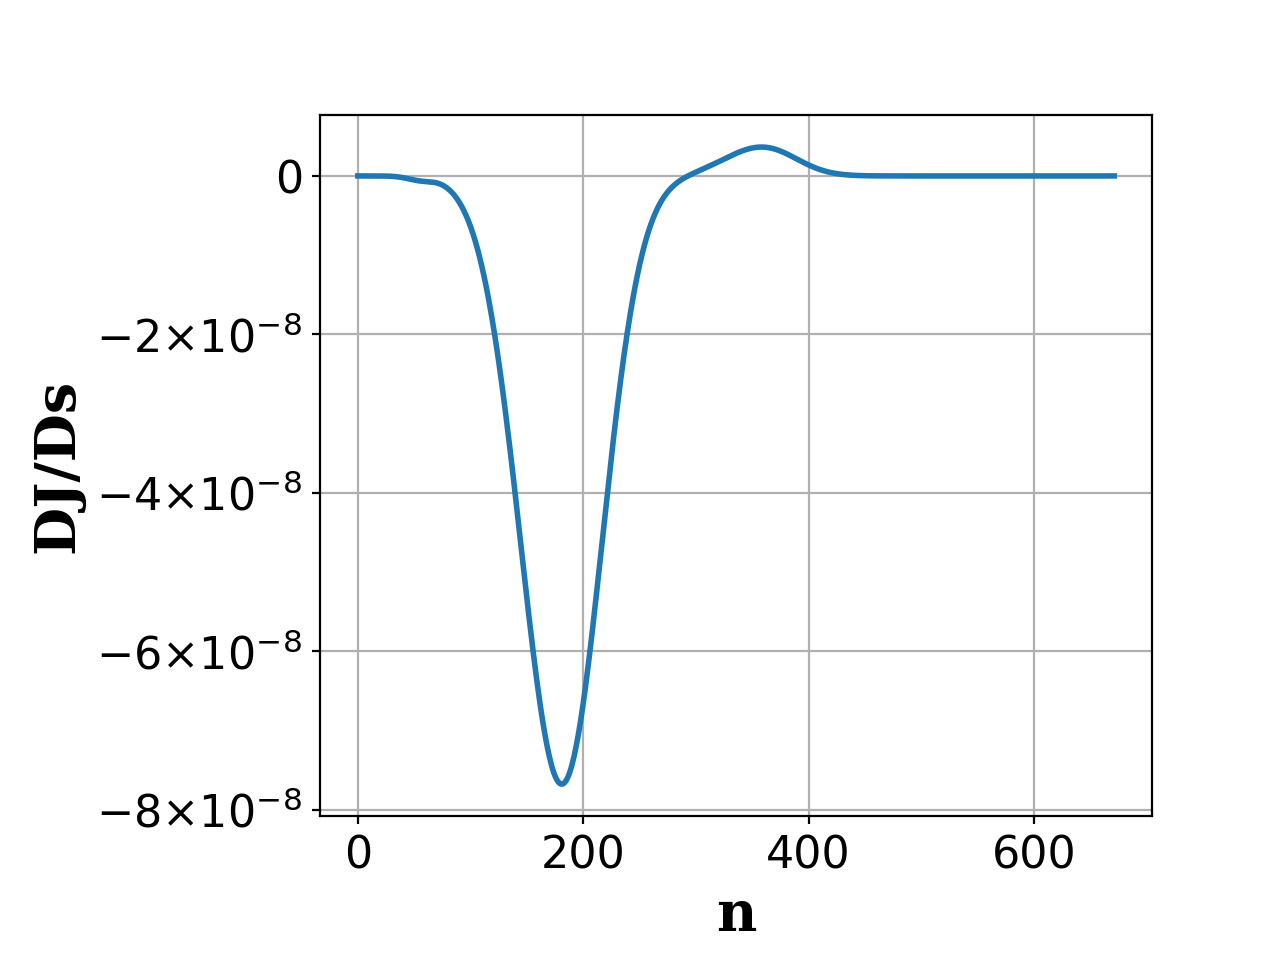
\includegraphics[width=0.5\textwidth]{figures/totdJdS.png}
  \caption{Adjoint solution at $t=2$}
  \label{fig:dJdS}
\end{figure}

\begin{table}[h]
  \begin{center}
    \caption[]{Comparison of $DJDs$ between adjoint-based approach and finite difference} \label{tb:comp}
    \begin{tabular}{p{0.05\textwidth}p{0.25\textwidth}p{0.25\textwidth}p{0.25\textwidth}}
      \hline
      n&      adjoint    & FD       & diff(\%)\\
      \hline
      200 & -6.649642178447126e-8 & -6.650801120737715e-8& 0.0174286414139 \\
      201 & -6.547562653134201e-8 & -6.548721076713906e-8& 0.0176924397837 \\
      202 & -6.441868649339054e-8 & -6.443026535579894e-8& 0.01797438451276 \\
      203 & -6.332777721431136e-8 & -6.333935056083499e-8& 0.01827530829712 \\
      204 & -6.220512517227239e-8 & -6.221669284582214e-8& 0.0185960136206 \\
      205 & -6.105300004457184e-8 & -6.106456191230011e-8& 0.01893742767731  \\
      \hline
    \end{tabular}
  \end{center}
\end{table}

\bibliographystyle{aiaa}
%\bibliography{reference}
\end{document}

